\documentclass[border=1mm]{standalone}
% \usepackage[margin=2.5cm]{geometry}

\usepackage{graphicx,tikz,tikz-layers,amsmath,ifthen,tabularray} 
\usetikzlibrary{decorations.markings,calc,positioning,arrows,shapes.geometric,arrows.meta,matrix,decorations.pathreplacing}

\usepackage[dvipsnames]{xcolor}

\colorlet{myred}{red!80!black}
\colorlet{myblue}{blue!80!black}
\colorlet{mybluee}{myblue!80!black}
\colorlet{mygreen}{green!60!black}
\colorlet{myorange}{orange!70!red!60!black}
\colorlet{mydarkred}{red!20!black}
\colorlet{mydarkblue}{blue!40!black}
\colorlet{mydarkgreen}{green!20!black}




\begin{document}

% \resizebox{\textwidth}{!}{
\tikz[font=\small, scale=1, every node/.style={outer sep=0pt, inner sep=0pt}, w/.style={minimum width=#1}, h/.style={minimum height=#1}, s/.style={minimum size=#1}, eu/.style={shorten >=#1}, ed/.style={shorten <=#1}, line join=round]
{
\tikzset{>={Latex[length=1.5mm, width=1.25mm]}}


\node[] (image1) {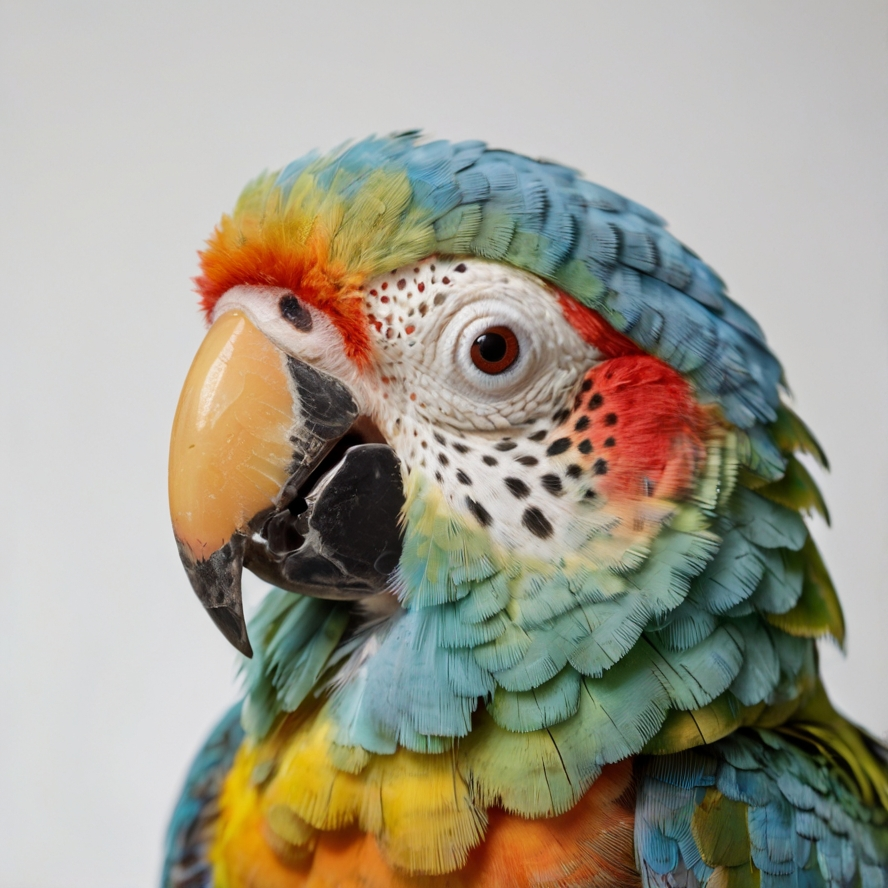
\includegraphics[width=1.5cm]{images/parrot3.jpg}};

\node[right=.65cm of image1, w=.8cm, h=1.5cm] (e) {$E$};
\begin{scope}[on behind layer]
 \draw[fill=myblue!15] (e.north west)--(e.south west)--($(e.south east)+(0,.15)$)--($(e.north east)+(0,-.15)$)--cycle;   
\end{scope}

\matrix[nodes={minimum width=2.5mm, minimum height=2.5mm}, row sep=0.3pt, column sep=0.3pt, right=.65cm of e, label={[label distance=2mm]below:$z_0$}] (mat1) {
    \node[fill=red] {}; & \node[fill=blue] {}; & \node[fill=green] {}; & \node[fill=yellow] {}; \\
    \node[fill=purple] {}; & \node[fill=orange] {}; & \node[fill=cyan] {}; & \node[fill=magenta] {}; \\
    \node[fill=brown] {}; & \node[fill=pink] {}; & \node[fill=gray] {}; & \node[fill=olive] {}; \\
    \node[fill=teal] {}; & \node[fill=lime] {}; & \node[fill=violet] {}; & \node[fill=black!20] {}; \\
};  

\node[draw, w=4.25cm, h=.7cm, fill=mygreen!15, right=3.5cm of mat1] (fdp) {Forward Diffusion Process};

\matrix[nodes={minimum width=2.5mm, minimum height=2.5mm}, row sep=0.3pt, column sep=0.3pt, right=3.5cm of fdp, label={[label distance=2mm]below:$z_T$}] (mat2) {
     \node[fill=teal] {}; & \node[fill=green] {}; & \node[fill=orange] {}; & \node[fill=cyan] {}; \\
    \node[fill=green] {}; & \node[fill=yellow] {}; & \node[fill=purple] {}; & \node[fill=brown] {}; \\
    \node[fill=white] {}; & \node[fill=lime] {}; & \node[fill=teal] {}; & \node[fill=pink] {}; \\
    \node[fill=gray] {}; & \node[fill=magenta] {}; & \node[fill=olive] {}; & \node[fill=black] {}; \\
};

%-------------------------------
\node[below=2cm of image1] (image2) {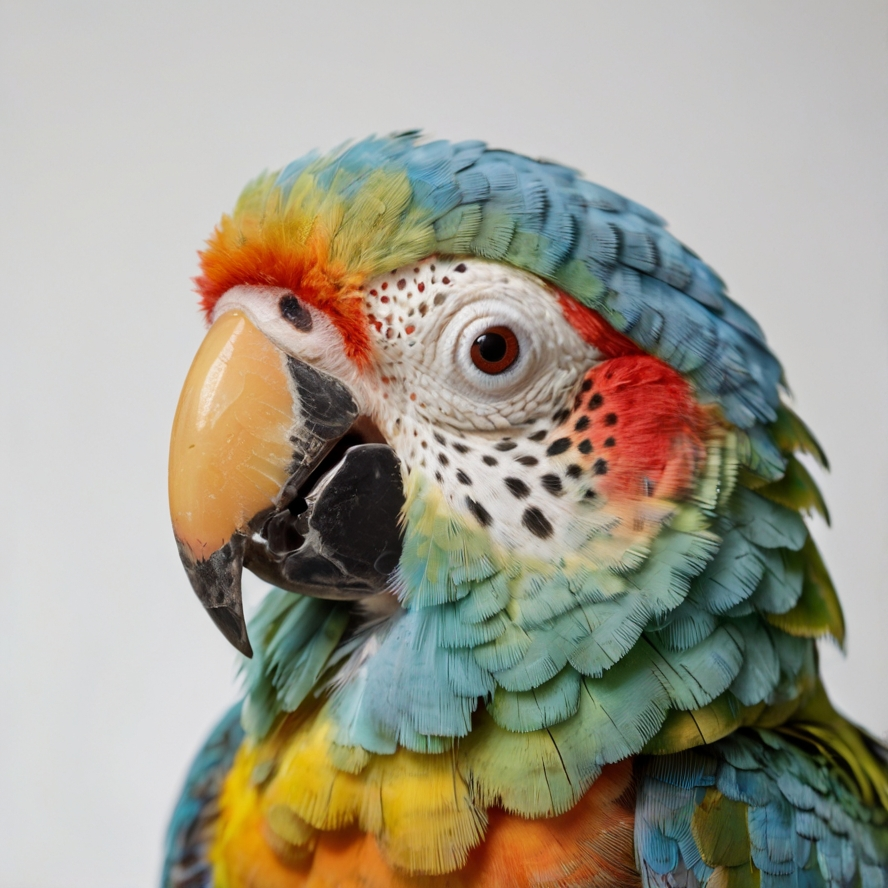
\includegraphics[width=1.5cm]{images/parrot3.jpg}};

\node[right=.65cm of image2, w=.8cm, h=1.5cm] (d) {$D$};
\begin{scope}[on behind layer]
 \draw[fill=myblue!15] (d.north west)--(d.south west)--($(d.south east)+(0,.15)$)--($(d.north east)+(0,-.15)$)--cycle;   
\end{scope}

\matrix[nodes={minimum width=2.5mm, minimum height=2.5mm}, row sep=0.3pt, column sep=0.3pt, right=.65cm of d, label={[label distance=2mm]below:$z_0$}] (mat3) {
    \node[fill=red] {}; & \node[fill=blue] {}; & \node[fill=green] {}; & \node[fill=yellow] {}; \\
    \node[fill=purple] {}; & \node[fill=orange] {}; & \node[fill=cyan] {}; & \node[fill=magenta] {}; \\
    \node[fill=brown] {}; & \node[fill=pink] {}; & \node[fill=gray] {}; & \node[fill=olive] {}; \\
    \node[fill=teal] {}; & \node[fill=lime] {}; & \node[fill=violet] {}; & \node[fill=black!20] {}; \\
};  

\matrix[nodes={minimum width=2.5mm, minimum height=2.5mm}, row sep=0.3pt, column sep=0.3pt, label={[label distance=2mm]below:$z_T$}] (mat4) at (mat3-|mat2) {
     \node[fill=teal] {}; & \node[fill=green] {}; & \node[fill=orange] {}; & \node[fill=cyan] {}; \\
    \node[fill=green] {}; & \node[fill=yellow] {}; & \node[fill=purple] {}; & \node[fill=brown] {}; \\
    \node[fill=white] {}; & \node[fill=lime] {}; & \node[fill=teal] {}; & \node[fill=pink] {}; \\
    \node[fill=gray] {}; & \node[fill=magenta] {}; & \node[fill=olive] {}; & \node[fill=black] {}; \\
};

\node[draw, w=1.5cm, h=1cm, fill=mygreen!15, right=1cm of mat3, label={[label distance=2mm]above:UNet}] (unet1) {};
\node[draw, w=1.5cm, h=1cm, fill=mygreen!15, left=1cm of mat4, label={[label distance=2mm]above:UNet}] (unet2) {};

\matrix[nodes={minimum width=2.5mm, minimum height=2.5mm}, row sep=0.3pt, column sep=0.3pt, label={[label distance=2mm]below:$z_1$}, right=.65cm of unet1] (mat5) {
     \node[fill=teal] {}; & \node[fill=cyan!70!violet] {}; & \node[fill=orange] {}; & \node[fill=pink] {}; \\
    \node[fill=violet!50] {}; & \node[fill=yellow!50!teal] {}; & \node[fill=purple] {}; & \node[fill=green] {}; \\
    \node[fill=violet] {}; & \node[fill=lime] {}; & \node[fill=teal] {}; & \node[fill=pink] {}; \\
    \node[fill=cyan] {}; & \node[fill=magenta] {}; & \node[fill=olive] {}; & \node[fill=cyan!50!green] {}; \\
};

\matrix[nodes={minimum width=2.5mm, minimum height=2.5mm}, row sep=0.3pt, column sep=0.3pt, label={[label distance=2mm]below:$z_{T-1}$}, left=.65cm of unet2] (mat6) {
     \node[fill=blue] {}; & \node[fill=purple] {}; & \node[fill=orange] {}; & \node[fill=red!50!blue] {}; \\
    \node[fill=green] {}; & \node[fill=green!50!violet] {}; & \node[fill=violet] {}; & \node[fill=brown] {}; \\
    \node[fill=lime] {}; & \node[fill=pink] {}; & \node[fill=teal] {}; & \node[fill=cyan] {}; \\
    \node[fill=gray] {}; & \node[fill=magenta] {}; & \node[fill=blue!50!green] {}; & \node[fill=blue] {}; \\
};


\node[draw=gray, anchor=south east, s=.2cm, fill=pink] (n1) at ($(mat5.north east)+(-.5pt,.2)$) {};
\node[draw=gray, anchor=south east, s=.2cm, fill=blue!20, left=0mm of n1] (n2) {};
\node[draw=gray, anchor=south east, s=.2cm, fill=cyan!20, left=0mm of n2, label={[label distance=1mm, font=\scriptsize]above:$t=1$}] (n3) {};
\node[draw=gray, anchor=south east, s=.2cm, fill=teal!20, left=0mm of n3] (n4) {};
\node[draw=gray, anchor=south east, s=.2cm, fill=orange!20, left=0mm of n4] (n5) {};
\draw[->, rounded corners=.5mm] (n5)--++(-.4,0) |- (unet1.15);
%--
\node[draw=gray, anchor=south east, s=.2cm, fill=pink] (n1) at ($(mat6.north east)+(-.5pt,.2)$) {};
\node[draw=gray, anchor=south east, s=.2cm, fill=blue!20, left=0mm of n1] (n2) {};
\node[draw=gray, anchor=south east, s=.2cm, fill=cyan!20, left=0mm of n2, label={[label distance=1mm, font=\scriptsize]above:$t\!=\!T\!-\!1$}] (n3) {};
\node[draw=gray, anchor=south east, s=.2cm, fill=teal!20, left=0mm of n3] (n4) {};
\node[draw=gray, anchor=south east, s=.2cm, fill=orange!20, left=0mm of n4] (n5) {};
%---
\node[draw=gray, anchor=south east, s=.2cm, fill=pink] (n1) at ($(mat4.north east)+(-.5pt,.2)$) {};
\node[draw=gray, anchor=south east, s=.2cm, fill=blue!20, left=0mm of n1] (n2) {};
\node[draw=gray, anchor=south east, s=.2cm, fill=cyan!20, left=0mm of n2, label={[label distance=1mm, font=\scriptsize]above:$t=T$}] (n3) {};
\node[draw=gray, anchor=south east, s=.2cm, fill=teal!20, left=0mm of n3] (n4) {};
\node[draw=gray, anchor=south east, s=.2cm, fill=orange!20, left=0mm of n4] (n5) {};
\draw[->, rounded corners=.5mm] (n5)--++(-.4,0) |- (unet2.15);
%---
\begin{scope}[on behind layer]
\draw[fill=mygreen!50!gray!5] ($(mat1.north east)+(.5,.25)$) rectangle ($(mat4.south west)+(-.5,-.5)$);    
\end{scope}

% \node[draw, fill=gray!10, anchor=north west, w=2.5cm, h=5.28cm] (box) at ($(mat2.north east)+(.5,.25)$) {};

% \node[w=2.25cm, h=.6cm, anchor=north] (co) at (box.north) {Conditioning};
% \node[draw, w=2.25cm, h=.6cm, below=1mm of co, fill=myred!15] (sm) {Semantic Map};
% \node[draw, w=2.25cm, h=.6cm, below=1mm of sm, fill=orange!15] (te) {Text};
% \node[draw, w=2.25cm, h=.6cm, below=1mm of te, fill=mygreen!15] (re) {\footnotesize Representations};
% \node[draw, w=2.25cm, h=.6cm, below=1mm of re, fill=myblue!15] (im) {Images};

% \begin{scope}[on above layer]
% \node[below=.6cm of im, h=.8cm, w=1.5cm] (tau) {$\tau_\theta$};    
% \end{scope}
% \draw[fill=myblue!15] (tau.north west)--(tau.north east)--($(tau.south east)+(-.15,0)$)--($(tau.south west)+(.15,0)$)--cycle;   


\node[draw, fill=gray!10, anchor=north west, w=9.75cm, h=3.2cm, xshift=-12cm, yshift=-6cm] (box) at ($(mat2.north east)+(.5,.25)$) {};

\node[w=2.25cm, h=.6cm, yshift=0.3cm] (co) at (box.south) {Conditioning};
\node[draw, w=2.25cm, h=.6cm, above=1mm of co, fill=myred!15, xshift=-3.5cm] (sm) {Semantic Map};
\node[draw, w=2.25cm, h=.6cm, right=1mm of sm, fill=orange!15] (te) {Text};
\node[draw, w=2.25cm, h=.6cm, right=1mm of te, fill=mygreen!15] (re) {\footnotesize Representations};
\node[draw, w=2.25cm, h=.6cm, right=1mm of re, fill=myblue!15] (im) {Images};

\begin{scope}[on above layer]
\node[above=1.5cm of co, h=.8cm, w=1.5cm, xshift=0.03cm] (tau) {$\tau_\theta$};    
\end{scope}
\draw[fill=myblue!15, rotate=180] (tau.north west)--(tau.north east)--($(tau.south east)+(-.15,0)$)--($(tau.south west)+(.15,0)$)--cycle;   



\draw[decorate, decoration={brace, amplitude=7pt}] 
        ($(sm.north west)+(0,1mm)$) -- ($(im.north east)+(0,1mm)$) 
        coordinate[pos=.5, yshift=7pt] (u);

\draw[decorate, decoration={brace, amplitude=7pt}] 
        ($(unet1.north west)+(0,1)$) -- ($(unet2.north east)+(0,1)$) 
        node[above=3mm,pos=.5] {Repeat $T$ times};

\foreach \i in {unet1,unet2}
{\node[w=1cm, h=1.5cm, scale=.5] (tra1) at ($(\i)+(-.35,0)$) {};
\begin{scope}[on above layer]
 \draw[fill=myblue!15] (tra1.north west)--(tra1.south west)--($(tra1.south east)+(0,.15)$)--($(tra1.north east)+(0,-.15)$)--cycle;   
 \node[draw, circle, s=.35cm, fill=orange!20] at (tra1) {};
\end{scope}

\node[w=1cm, h=1.5cm, scale=.5] (tra1) at ($(\i)+(.35,0)$) {};
\begin{scope}[on above layer]
 \draw[fill=myblue!15] (tra1.north east)--(tra1.south east)--($(tra1.south west)+(0,.15)$)--($(tra1.north west)+(0,-.15)$)--cycle;   
 \node[draw, circle, s=.35cm, fill=orange!20] at (tra1) {};
\end{scope}}



% Arrows
\draw[->] (u)--(tau);
\draw[->, rounded corners=1mm] (tau.north)--coordinate[pos=1] (z) ++(0,.75) -| (unet1);
\draw[->, rounded corners=1mm] (tau.north)--coordinate[pos=1] (z) ++(0,.75) -| (unet2);
\draw[->] (image1)--(e); 
\draw[->] (e)--(mat1);
\draw[->] (mat1)--(fdp)--(mat2);

\draw[->] (mat4)--(unet2);
\draw[->] (unet2)--(mat6);
\draw[->] (mat6)--node[fill=white, w=1cm] {\large$\ldots$} (mat5);
\draw[->] (mat5)--(unet1);
\draw[->] (unet1)--(mat3);
\draw[->] (mat3)--(d);
\draw[->] (d)--(image2);

}

% }



\end{document}
